\chapter{Experiment}
    This chapter describes about experimental setup in this study. The experiment is performed at Rare Isotope Beam Factory (RIBF) at RIKEN Nishina Center.\cite{RIKEN} A primary ${}^{48}$Ca beam is produced by the RIKEN accelerator complex and delivered to the BigRIPS separator. \cite{Kubo03} \cite{Kubo07} \cite{Kubo12} The BigRIPS separator produced the ${}^{17}$B secondary beam which bombarded on the lead and carbon targets in front of the SAMURAI (Superconducting Analyzer for MUlti-particles from Radioisotope beams) spectrometer. \cite{SAMURAI} After the reaction at target, the fragments ${}^{15}$B and two neutrons are detected by detectors at SAMURAI area. Note that this experiment was part of the SAMURAI Dayone experiment which was the first physics run using the SAMURAI spectrometer.

\section{BigRIPS separator}

    \begin{figure}
        \centering
        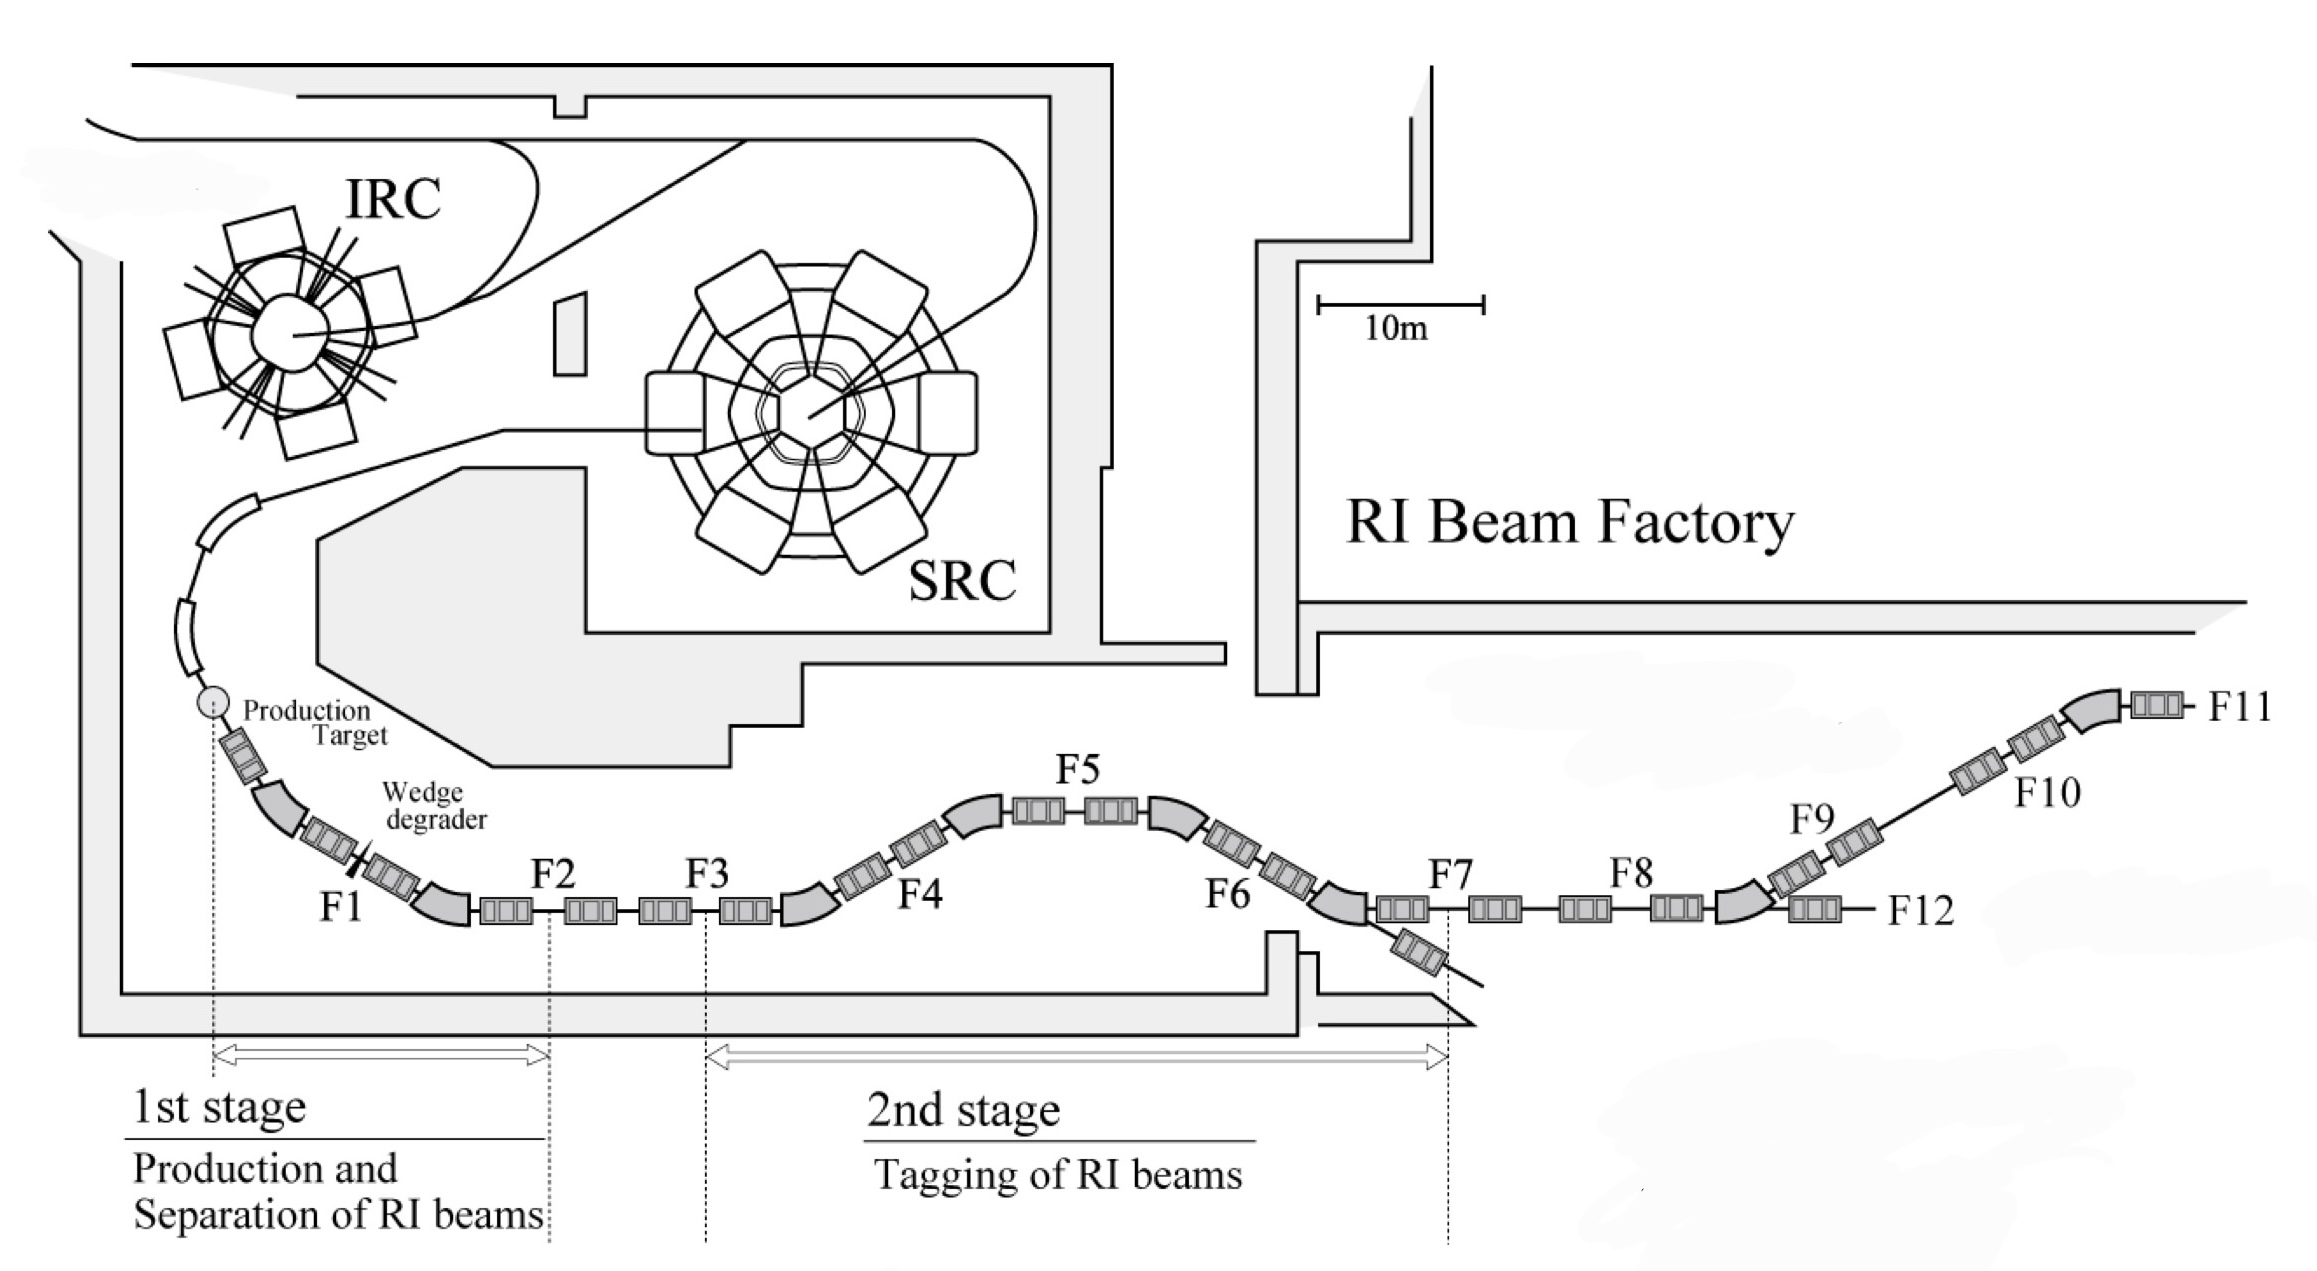
\includegraphics[width=12cm]{chapter3/BigRIPS_roof.jpg}
        \caption{A top view of the BigRIPS separator}
    \end{figure} 

After primary ${}^{48}$Ca beam is produced at SRC accelerator, the beam bombarded on a 30mm thick Be target and the secondary beam is produced through the in-flight fragmentation method. Since the secondary beam includes many rare isotopes, the RI beam is separated by the BigRIPS separator. Table 3.1 shows the BigRIPS separator setup for Dayone experiment. In the first stage of BigRIPS separator, the RI beam separated by dipole magnet with slit and wedge-shaped degrader located at F1 focal plane. In the dipole magnet, the rigidity of a particle can be written as following eq \ref{eq:rigidity}.
    \begin{align}
        \rho = \frac{A}{Z} \cdot\frac{v}{B} \label{eq:rigidity}
    \end{align}
The velocity of the secondary beam is almost same regardless of the nuclei so that it can be possible to choose specific $A/Z$ by adjusting the slit to filter only some $B\rho$ value. After that, the wedge-shaped degrader makes the beam energy depends on the $Z$ so that even same $A/Z$ nuclei can be separated. In the second stage, the RI beam is identified using TOF-B$\rho$-$\Delta E$ method. Each detector information will be described as following.
    \begin{table}[h]
        \centering
        \begin{tabular}{c c c c}
            \hline
            Focal Plane & Dipole Magnet [Tm] & Slit[mm] & Degrader / Detector \\
            \hline
            F0  & 9.1734 &  & Be target (30mm) \\
            F1  & 8.8195 & $\pm$120 & Al wedge degrader \\
            F2  & 8.8195 & L: 10 R: 7 & \\
            F3  & 8.7841 &  & Plastic Scintillator (3mm)\\
            F5  & 8.780  & $\pm$120 & BPC \\
            F7  & 8.780  & $\pm$120 & Plastic Scintillator (3mm)\\
            %F13 &  & & Plastic Scintillator (0.5mm$\times$2)\\
            \hline
        \end{tabular}
        \caption{BigRIPS separator setup for Dayone experiment \cite{Dayonelog}}
    \end{table}

\subsection{Plastic Scintillator}
At focal plane F3, F7, F13, plastic scintillators are located for measuring the time of flight (TOF) of secondary beam. In F3 and F7, plastic scintillator with 3mm thickness is located and at F13 there are two scintillators, SBT1 and SBT2, with 0.5mm thickness. The flight length between F7 and F13 (Average point of SBTs) is 3662.00mm.

\begin{table}[h]
    \centering
    \begin{tabular}{c|ccc}
        \hline
        & Location & Thickness & Distance from target upstream \\
        \hline
        SF3 & F3 & 3mm & 86053.56 mm\\
        SF7 & F7 & 3mm & 39483.58 mm\\
        SBT1 & F13 &0.5mm & 2904.08 mm\\
        SBT2 & F13 &0.5mm & 2824.08 mm\\
        \hline
    \end{tabular}
    \caption{Information of Plastic Scintillators at F3, F7, F13}
\end{table}


\subsection{BPC (Beam Proportional Chamber)}
BPC is Multi Wire Proportional Chamber (MWPC) located at F5 focal plane which is used for measuring the position of beam. The purpose of BPC is tagging magnetic rigidity and momentum of secondary beam.
\begin{table}[h]
    \centering
    \begin{tabular}{l|c}
        \hline
        Effective Area & (H)240mm x (V)150mm \\
        Configuration & $XX$ (2 Planes) \\
        number of wire & 64 $\times$ 2 = 128 \\
        Wire Pitch & 4mm \\
        Gas & $i$--${C}_{4} {H}_{10}$ at 50 torr\\
        \hline
    \end{tabular}
    \caption{Parameter of BPC (Beam Proportional Chamber) \cite{SAMURAI}}
\end{table}


\begin{figure}[h]
    \centering
    \begin{subfigure}[h]{\textwidth}
        \centering
        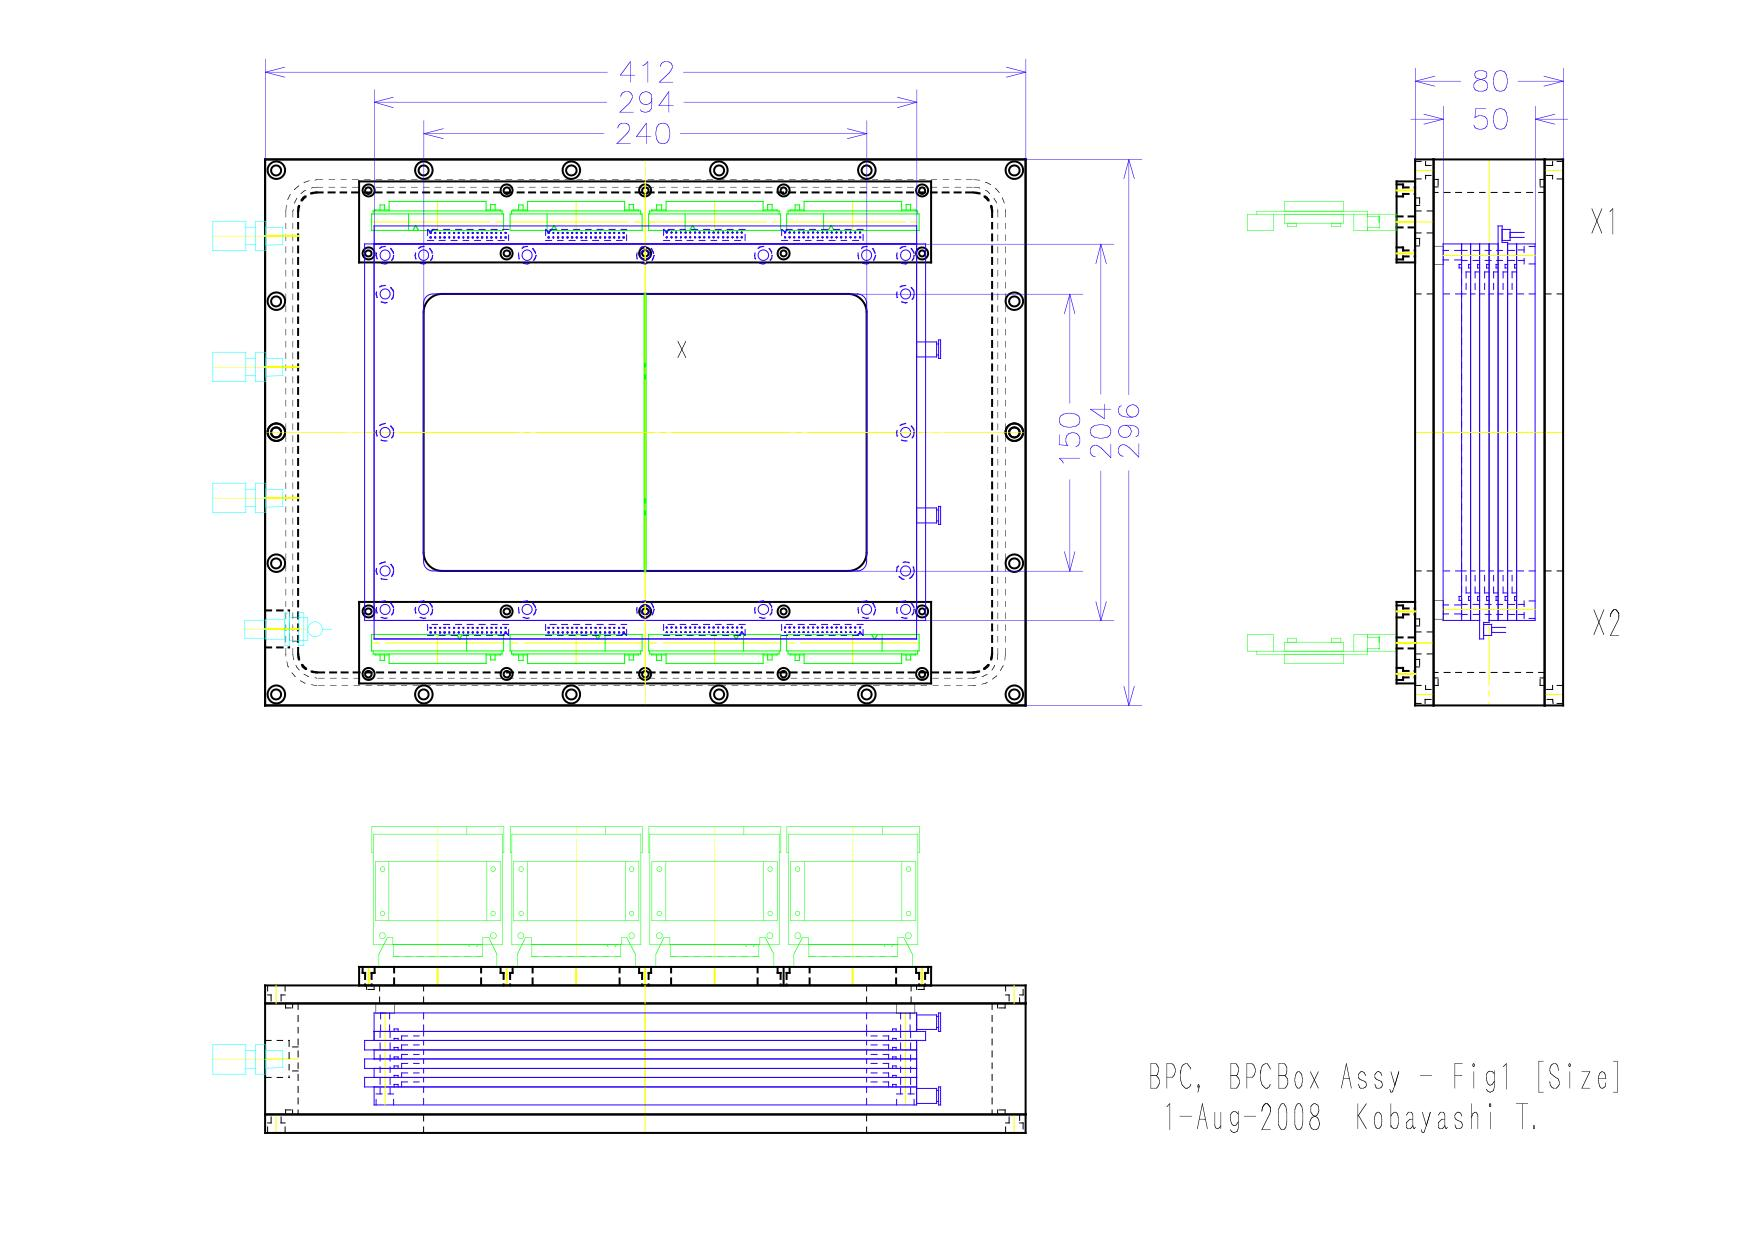
\includegraphics[width=12cm]{chapter3/bpc_a1.jpg}
    \end{subfigure}
    \begin{subfigure}[h]{\textwidth}
        \hspace{2.4cm}
        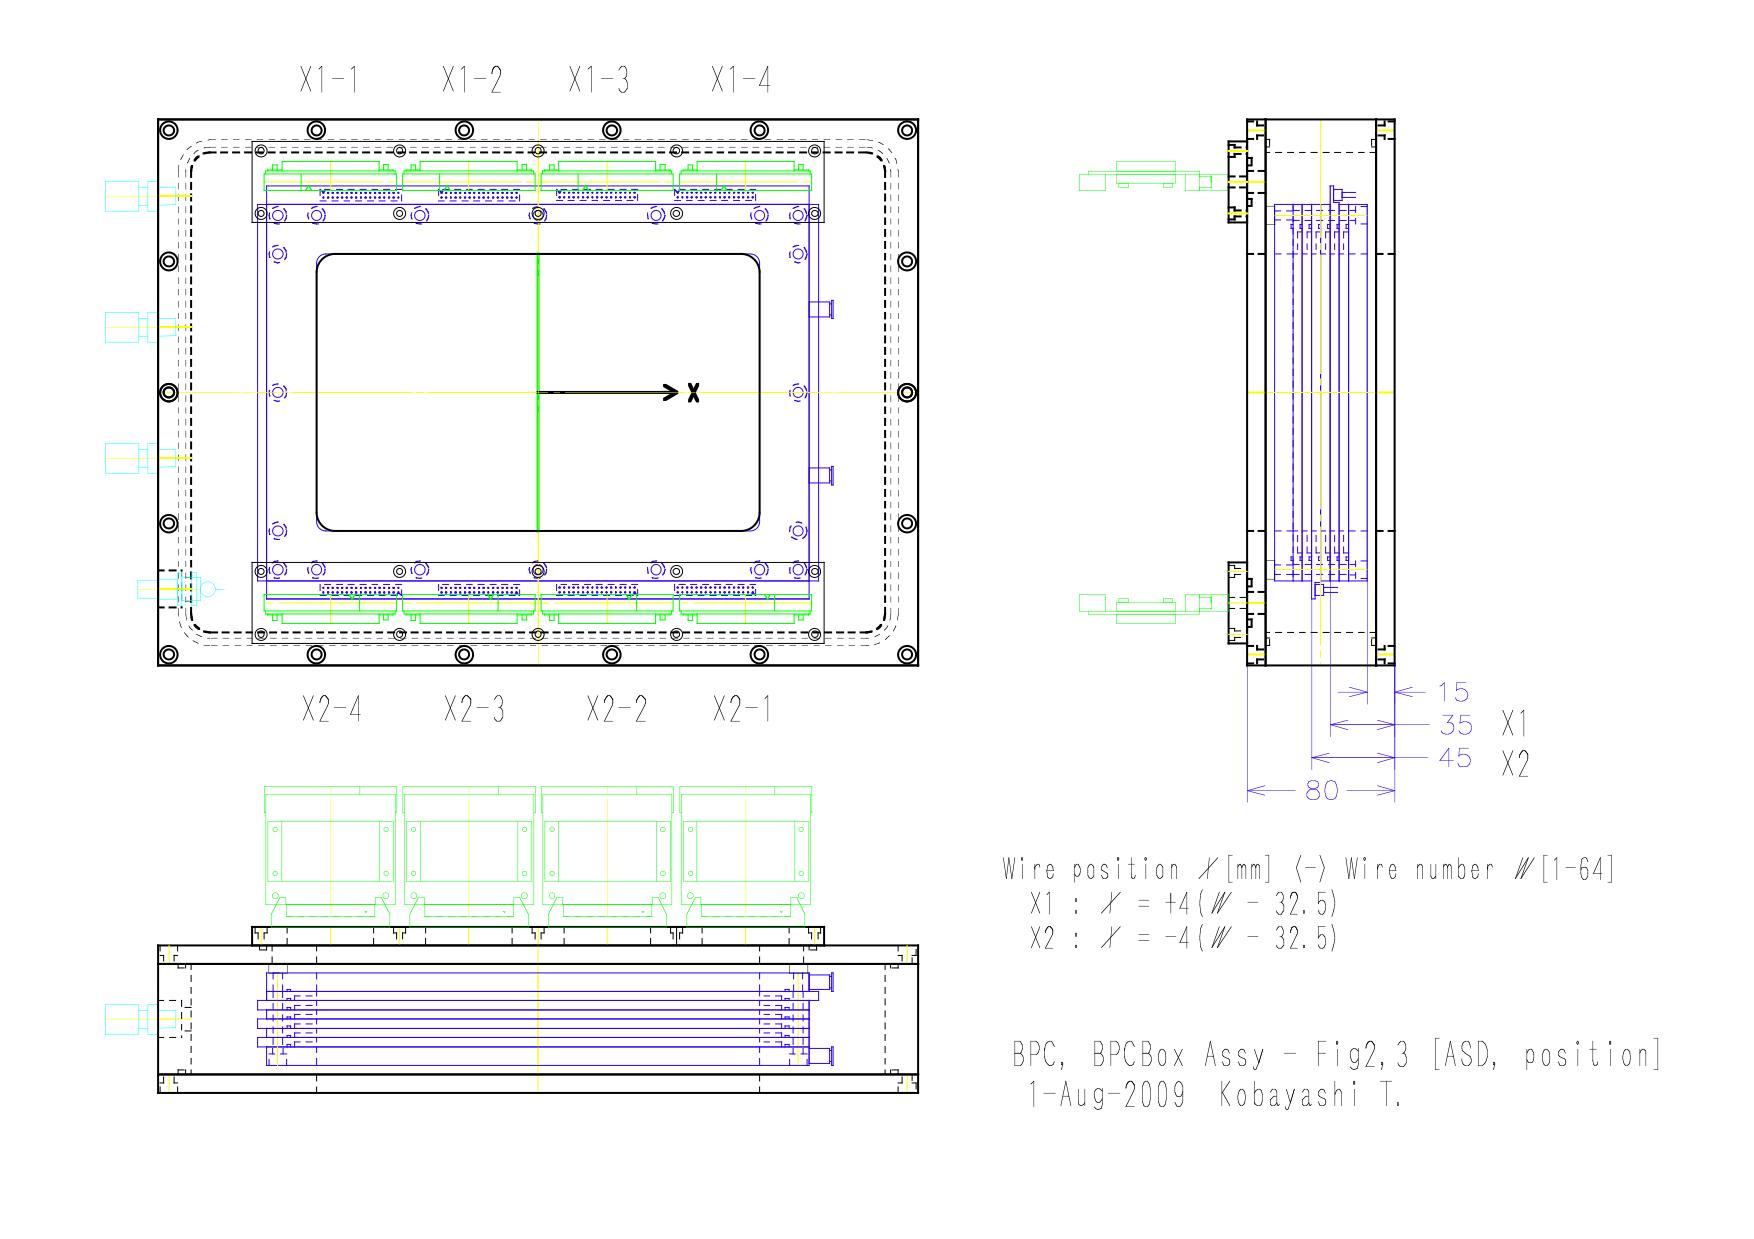
\includegraphics[width=12.5cm]{chapter3/bpc_a23.jpg}
    \end{subfigure}
        \caption{Schematic View of BPC (Beam Proportional Chamber) \cite{SAMURAI}}
\end{figure}

\clearpage

\subsection{ICB (Ion Chamber for Beam)}
The ICB is multi-layer ionization chamber for measuring the energy loss ($\Delta E$) of secondary beam. Using P10 gas at 1 atm, the energy loss of secondary beam can be measured. 
\begin{table}[h]
    \centering
    \begin{tabular}{l|c}
        \hline
        Effective Area & (H)140mm x (V)140mm x (D)420mm\\
        Configuration & 10 anodes and 11 cathodes \\
        Anode-cathode gap & 21mm \\
        Gas & P10 at 1 atm\\
        Distance from target upstream & 476.87 mm \\
        \hline
    \end{tabular}
    \caption{Parameter of ICB (Ion Chamber for Beam) \cite{SAMURAI}}
\end{table}

\begin{figure}[t]
    \centering
    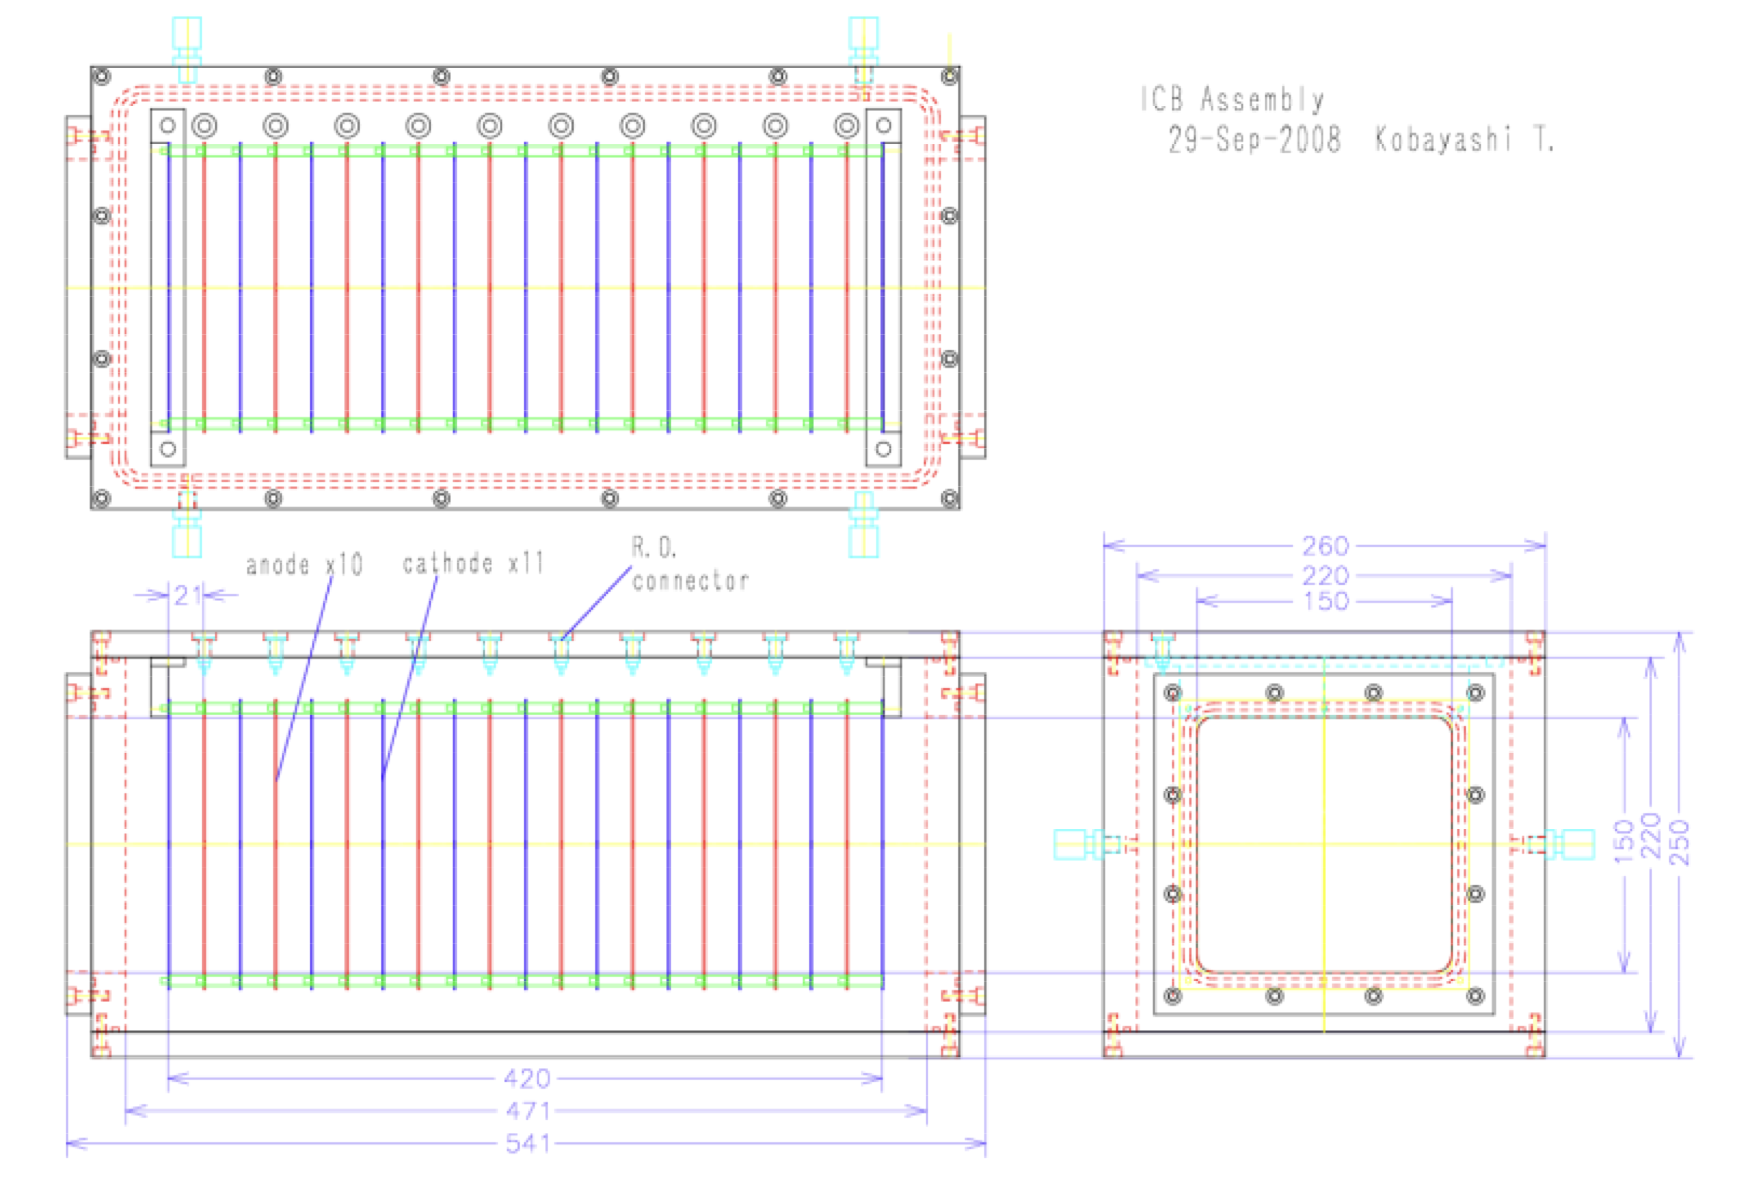
\includegraphics[width=11cm]{chapter3/icb_a}
    \caption{Schematic View of ICB (Ion Chamber for Beam) \cite{SAMURAI}}
\end{figure}

\subsection{BDC1, BDC2 (Beam Drift Chamber)}
Before target, there are two Beam drift chamber for reconstructing the trajectory of secondary beam. Using the trajectory information, the position of secondary beam at target can be calculated. In this experiment, each BDC box is filled with $i$--${C}_{4} {H}_{10}$ gas at 100 torr. 

\begin{table}[h]
    \centering
    \begin{tabular}[h]{l|c}
        \hline
        Effective Area & (H)80mm x (V)80mm\\
        Configuration & $XX'YY'XX'YY'$ (8 planes)\\
        Number of Wire & 16 $\times$ 8 = 128 \\
        Wire Pitch & 5mm \\
        Gas & $i$--${C}_{4} {H}_{10}$ at 100 torr\\
        Distance from target upstream & (BDC1) 2032.12mm (BDC2) 1032.8 mm \\
        \hline
    \end{tabular}
    \caption{Parameter of BDC (Beam Drift Chamber) \cite{SAMURAI}}
\end{table}

\begin{figure}[h]
    \centering
    \begin{subfigure}{\textwidth}
        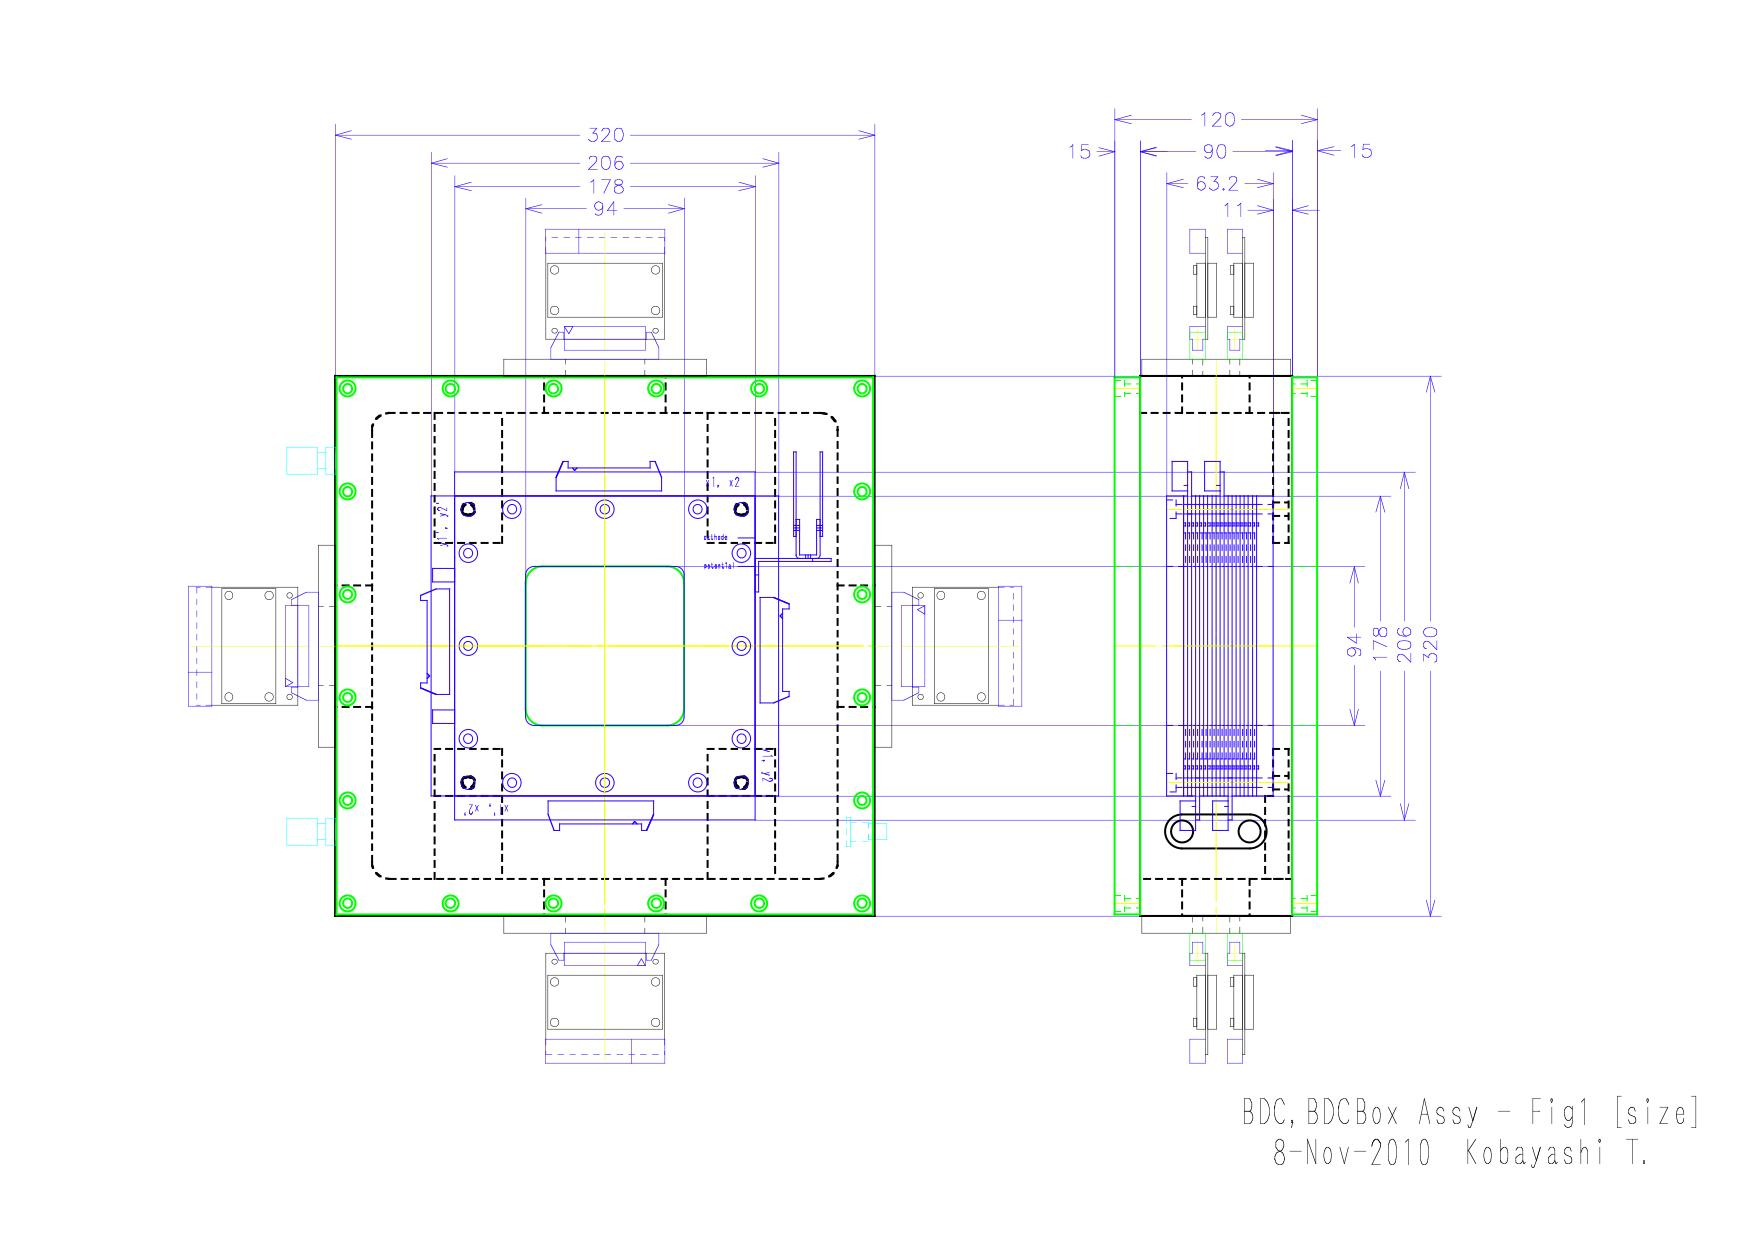
\includegraphics[width=12cm]{chapter3/bdc_a1.jpg}    
    \end{subfigure}
    \begin{subfigure}{\textwidth}
        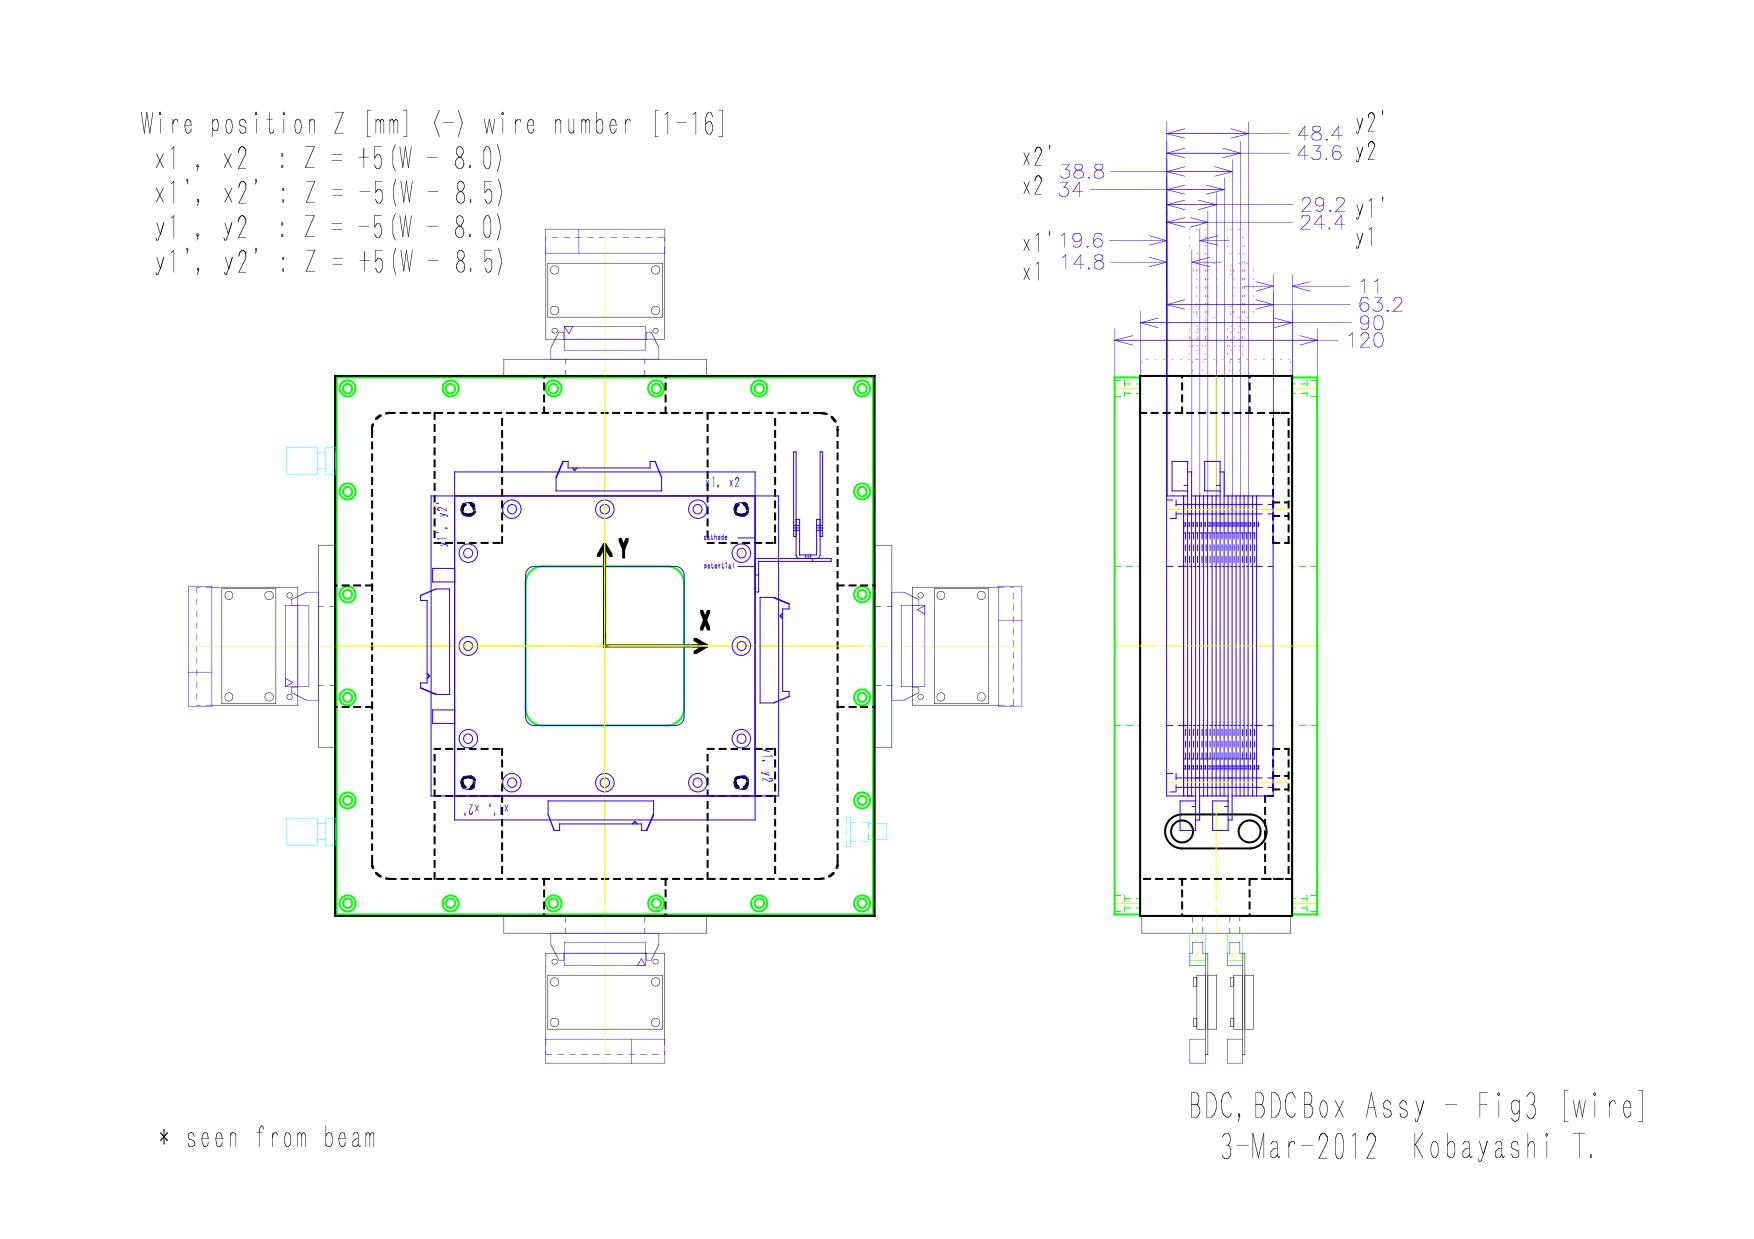
\includegraphics[width=12cm]{chapter3/bdc_a3.jpg}
    \end{subfigure}
    \caption{Schematic View of BDC (Beam Drift Chamber) \cite{SAMURAI}}
\end{figure}

\clearpage

\section{SAMURAI}

\begin{figure}[hbt!]
    \centering
    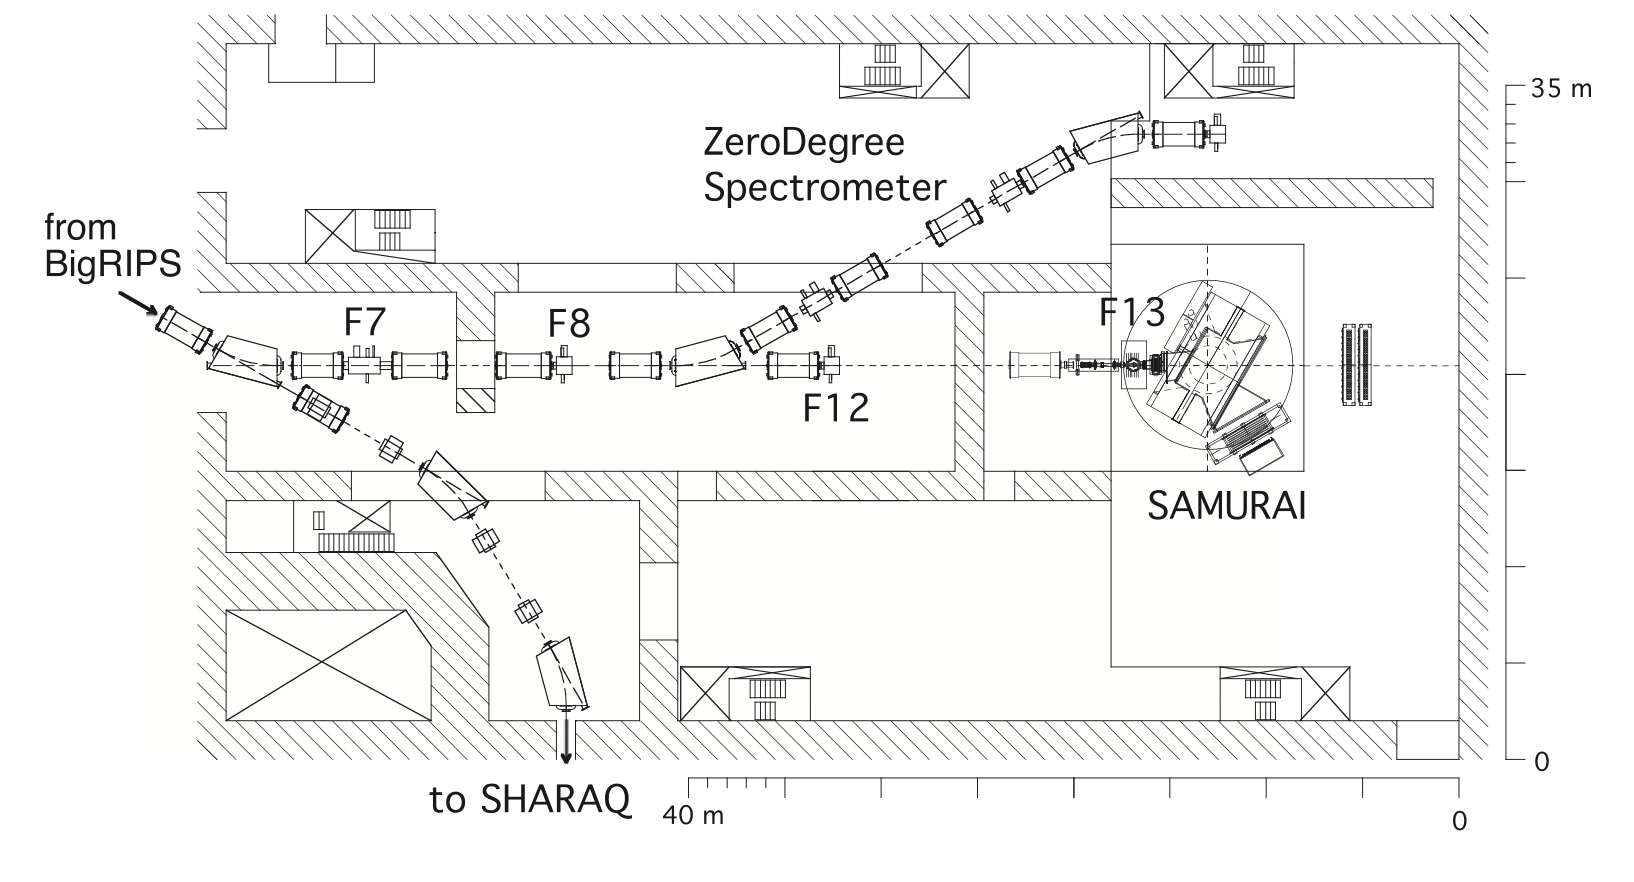
\includegraphics[width=12cm]{chapter3/SAMURAI1.png}
    \caption{A top view of the beam line from BigRIPS to SAMURAI spectrometer}
\end{figure}

The SAMURAI spectrometer is designed for kinematically complete experiment such as invariant mass spectroscopy. \cite{SAMURAIConcept} Charged fragment bent by SAMURAI superconducting magnet and detected by two drift chambers (FDC1, FDC2) and one plastic scintillator (HODF). Two drift chamber for fragment are located at before and after SAMURAI magnet, for rigidity analysis. And plastic scintillator HODF is placed after FDC2 to measure the TOF and energy loss of fragment. Finally the neutron detector array NEBULA is located at the end of extended beam line for neutron detection. Using SAMURAI system, the invariant mass of the system can be reconstructed by measuring all of the fragments and neutrons.

\begin{figure}[t]
    \centering
    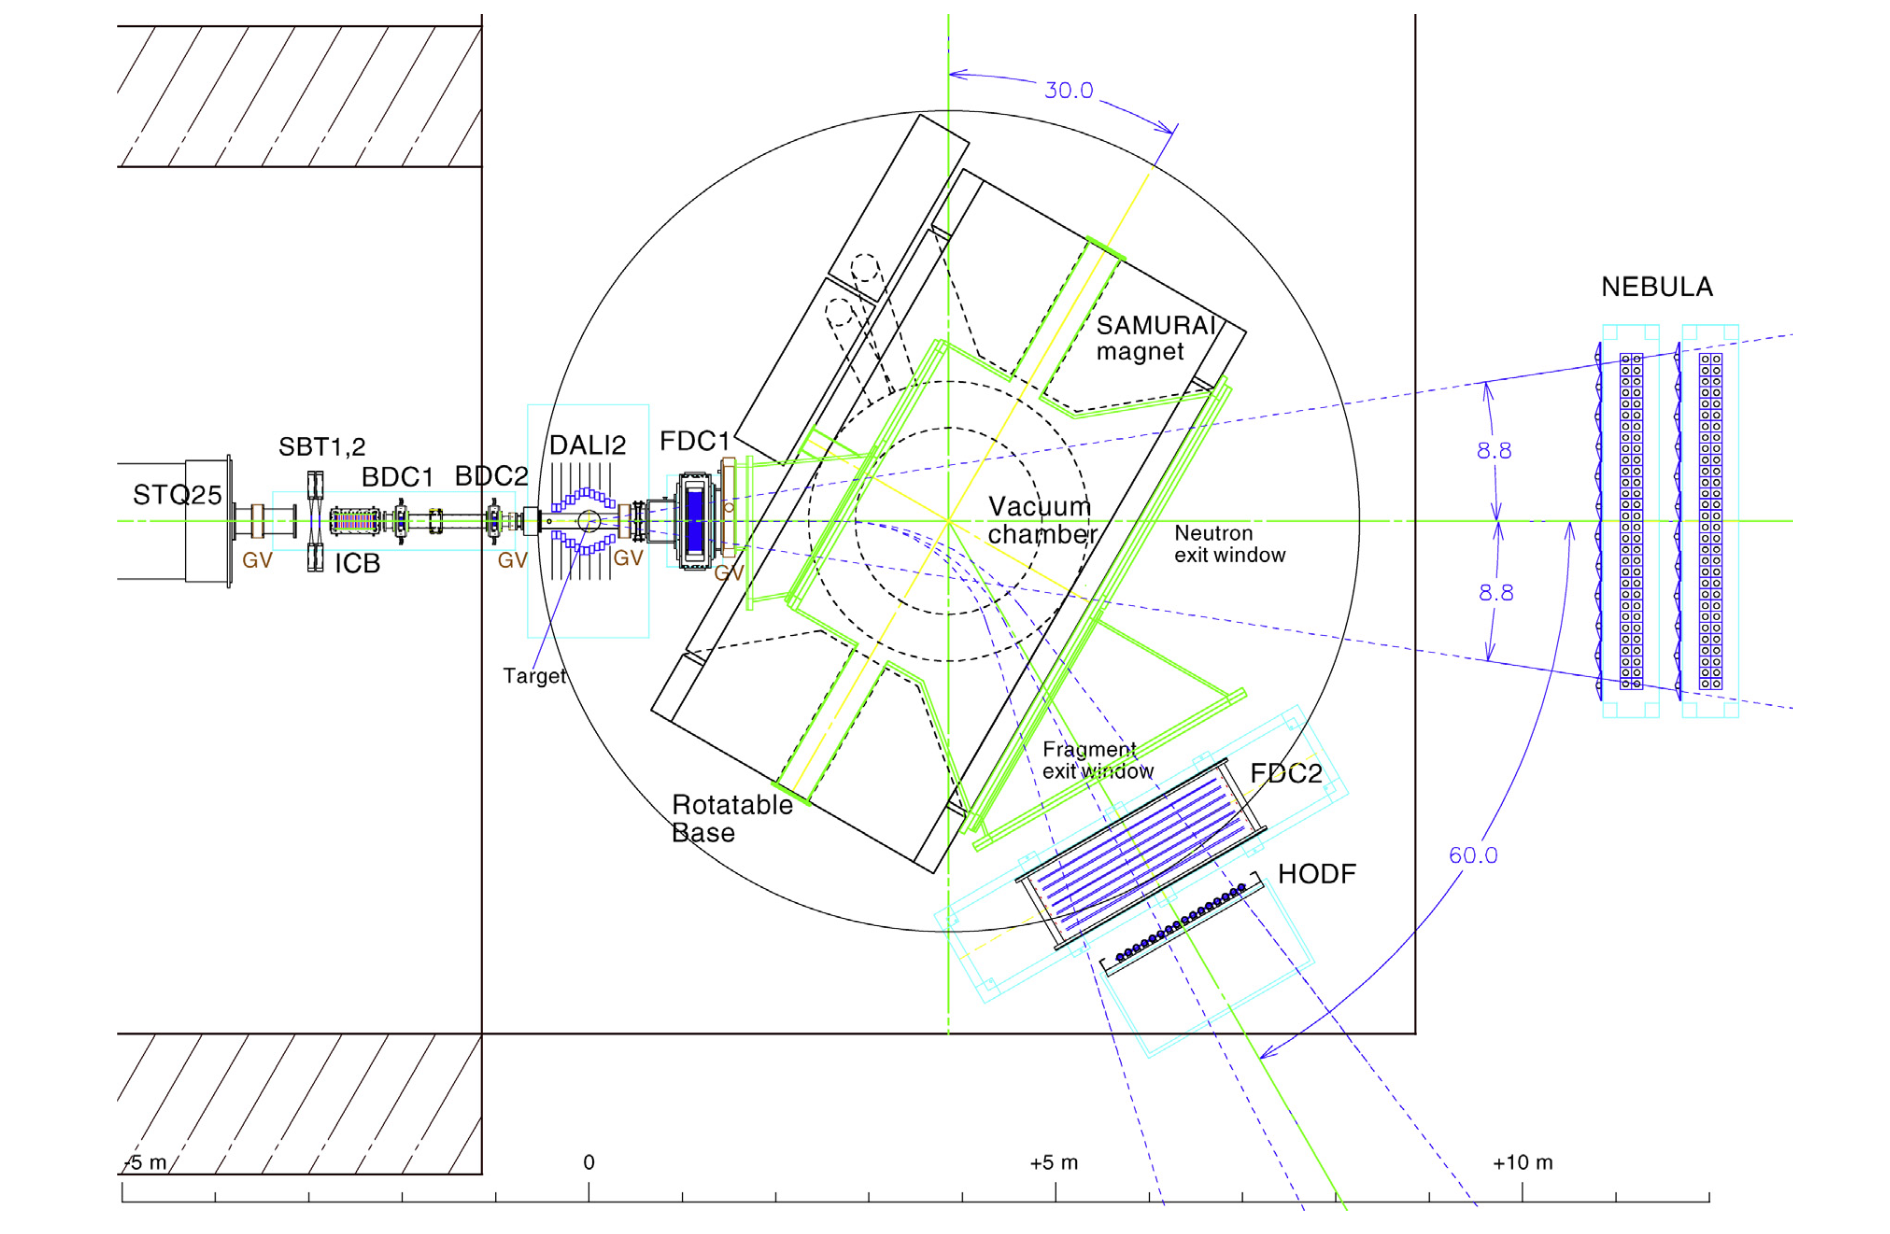
\includegraphics[width=12cm]{chapter3/SAMURAI.png}
    \caption{A top view of the SAMURAI spectrometer}
\end{figure}

\subsection{SAMURAI Magnet}

\begin{table}[h]
    \centering 
    \begin{tabular}{l|c}
    \hline
    Type & Superconducting dipole magnet \\
    Magnet Pole & $\phi$ 2m (0.88 m gap) \\
    Maximum field & 3.1 T \\
    Maximum current & 563 A \\
    Acceptance & $\theta_H \leq \pm 10{}^{\circ}$, $\theta_V \leq \pm 5{}^{\circ}$\\
    \hline
    \end{tabular}
    \caption{Parameter of SAMURAI Magnet \cite{SAMURAI}}
\end{table}

\subsection{FDC1, FDC2 (Forward Drift Chamber)}
After target, there are two Forward Drift Chamber for reconstructing the trajectory of charged fragment. Using the trajectory information, the rigidity of charged fragment at target can be calculated. In this experiment, FDC1 is filled with $i$--${C}_{4} {H}_{10}$ gas at 50 torr and FDC2 is filled with He + 50\% ${C}_{2} {H}_{6}$ gas at 1 atm. 

\begin{table}[h]
    \centering
    \begin{tabular}{l|c}
        \hline
        Effective Area & (H)400mm x (V)300mm x (D)180mm\\
        Configuration & $XX'UU'VV'XX'UU'VV'XX'$ (14 planes)\\
        Number of Wire & 32 $\times$ 14 = 448 \\
        Wire Pitch & 10mm \\
        Gas & $i$--${C}_{4} {H}_{10}$ at 50 torr\\
        Distance from target upstream & 1151.38 mm  \\
        \hline
    \end{tabular}
    \caption{Parameter of FDC1 (Forward Drift Chamber 1) \cite{SAMURAI}}
\end{table}

\begin{table}[h]
    \centering
    \begin{tabular}{l|c}
        \hline
        Effective Area & (H)2296mm x (V)836mm x (D)860mm\\
        Configuration & $XX'UU'VV'XX'UU'VV'XX'$ (14 planes)\\
        Number of Wire & 112 $\times$ 14 = 1568 \\
        Wire Pitch & 20mm \\
        Gas & He + 50\% ${C}_{2} {H}_{6}$ at 1 atm\\
        \hline
    \end{tabular}
    \caption{Parameter of FDC2 (Forward Drift Chamber 2) \cite{SAMURAI}}
\end{table}

\subsection{HODF (HODoscope for Fragment)}
The plastic scintillator HODscope is located behind FDC2 for measuring the TOF and energy loss of charged fragment. For the charged fragment identification, TOF-B$\rho$-$\Delta E$ method is used as same as beam particle identification at BigRIPS. For 
\begin{table}[h]
    \centering
    \begin{tabular}{l|c}
        \hline
        Effective Area & (H)1600mm x (V)1200mm x (D)10mm\\
        Number of Scintillator & 16 \\
        Width of Scintillator & 10mm \\
        \hline
    \end{tabular}
    \caption{Parameter of HODF (HODscope for Fragment) \cite{SAMURAI}}
\end{table}

\subsection{NEBULA}
For measuring momentum vector of neutron, 

\section{Electronics}
\subsection{Run summary}
\begin{center}
    \begin{tabular}[h]{c|ccc}
        \hline
        Run number& Target & Trigger & note\\
        \hline
        394 - 404 &  C (1.789 g/cm${}^{2}$)  & DSB(1/20) + B x N + D(1/1) &\\
        405 - 409 &  Empty  & DSB(1/20) + B x N + D(1/1) &\\
        410 - 427 &  Pb (3.255 g/cm${}^{2}$)  & DSB(1/20) + B x N + D(1/1) &\\
        428 - 431 & Pb (3.255 g/cm${}^{2}$)  & DSB(1/20) + B x N + D(1/1) & F5 slit $\pm$1mm \\
        \hline
    \end{tabular}
\end{center}

\subsection{Trigger condition}
There are four triggers condition which are used in this experiment; DSB, B$\times$N, B$\times$N, B$\times$N. They are defined as follows.
\begin{enumerate}
    \item \textbf{DBS} (Down Scale Beam) 
    \item \textbf{B$\times$N} (Coincidence between Beam and NEBULA)
    \item \textbf{B$\times$D} (Coincidence between Beam and DALI)
    \item \textbf{B$\times$H} (Coincidence between Beam and HODF)
\end{enumerate} 

\subsection{Live Time}
The DAQ readout rate is limited by the dead time of the DAQ sub-system. And the dead time depends on the trigger condition and the target.  
\begin{table}[h]
    \centering
    \begin{tabular}{c|c|cc}
        \hline
        Run number & target & DBS & B $\times$ N  \\
        \hline
        394 - 404 & C & 0.843 & 0.815 \\
        405 - 409 & Empty & 0.890 & 0.854 \\
        410 - 427 & Pb & 0.861 & 0.831 \\
        \hline
    \end{tabular}
    \caption{Live time of each reaction trigger}
\end{table}
